\documentclass[a4paper, 12pt]{article}

\usepackage[table,xcdraw]{xcolor}
\usepackage[left=2.5cm, right=1.5cm, top=1.5cm, bottom=1.5cm]{geometry}
\usepackage{graphicx}
\usepackage{xcolor}
\usepackage{mdframed}
\usepackage { amsmath , amssymb , amsthm }
\usepackage[T2A]{fontenc}
\usepackage[utf8]{inputenc}
\usepackage[english,russian]{babel}
\usepackage{listings}
\usepackage{setspace}
\usepackage{amsmath}
\usepackage{float}


\onehalfspacing
\renewcommand{\familydefault}{\sfdefault}
% \renewcommand{\familydefault}{\sffamily}

\graphicspath{{img/}}
\DeclareGraphicsExtensions{.pdf,.png,.jpg}


\begin{document}
\begin{titlepage}
  \begin{center}
    \MakeUppercase{Министерство науки и высшего образования Российской Федерации} \\
    \MakeUppercase{ФГБОУ ВО Алтайский госудаственный университет}
    \vspace{0.25cm}
    
	  Институт цифровых технологий, электроники и физики
    
    Кафедра вычислительной техники и электроники
    \vfill
    
    {\LARGE Отчёт по лабораторным работам. 13 вариант}\\[5mm]
    \textsc{(по курсу <<Методы оптимизации>>)}
  \bigskip

\end{center}
\vfill

\newlength{\ML}
\settowidth{\ML}{«\underline{\hspace{0.7cm}}» \underline{\hspace{1cm}}}
\hfill
\begin{minipage}{0.45\textwidth}
  Выполнил: ст. 595 гр.:\\
  \underline{\hspace{\ML}} Д.\,В.~Осипенко\\
  Проверил: к.ф-м. наук, доцент каф. ВТиЭ\\
  \underline{\hspace{\ML}} В.\,И.~Иордан\\
  «\underline{\hspace{0.7cm}}» \underline{\hspace{2cm}} \the\year~г.
\end{minipage}%
\vfill

\begin{center}
  Барнаул, \the\year~г.
\end{center}
\end{titlepage}
\tableofcontents
\newpage

\section{Графический метод решения задач линейного программирования}
\subsection{Краткие теоретические сведения по теме лабораторной работы}
Пусть необходимо найти максимальное значение функции $Z(x) =c_1x_1 + c_2x_2 $ при ограничениях:\\

\begin{math}
  \begin{cases}
    a_{11}x_1+a_{12}x_2 \leq b_1\\
    a_{21}x_1+a_{22}x_2 \leq b_2\\
    \ldots\\
    a_{m1}x_1+a_{m2}x_2 \leq b_m\\
  \end{cases}
  \quad
  x_1 \geq 0, x_2 \geq 0
\end{math}\\

Допустим, что система ограничений имеет решение, а ее многоугольник решений ограничен.

Каждое из неравенств ограничений определяет полуплоскость с границей $a_{i1}+x_1+a{i2}x_2 = b_i, i=1\ldots m$ или $x_1=0,x_2=0$

Так как множество точек пересечения данных полуплоскостей - выпуклое, то областью допустимых решений задачи является выпуклое множество, которое называется многоугольником решений. Стороны этого многоугольника лежат на прямых, уравнения которых получаются из исходной системы ограничений заменой знаков неравенств на знаки точных равенств.

Представим этот многоугольник на плоскости:\\
\begin{center}
  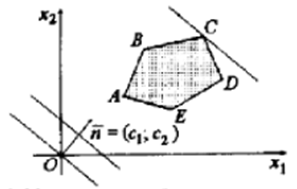
\includegraphics[]{1-2.png}\\
  Рис. 1.1. Многоугольник области допустимых решений\\
\end{center}

Линейная функция при фиксированных значениях $Z(x)=0$ является уравнением прямой линии $c_1x_1+c_2x_2=const$. Прямая, соответствующая данной функции, проходит через начало координат. Другим значениям соответствует прямые параллельные друг другу.

Прямая, уравнение которой получается из целевой функции, если ее приравнять постоянной величине, называется линией уровня.

Вектор нормали уровня $\vec{n}$ имеет координаты c1 и c2.

Если перемещать линию уровня параллельно своему начальному положению в направлении вектора $\vec{n}$, то последней точкой, в которой линия уровня коснется области допустимых решений (ОДР) будет точка с.

Линия уровня, имеющая общие точки с ОДР и расположенная так, что ОДР целиком находится в одной из полуплоскостей называется опорной прямой.

Алгоритм решения задачи линейного программирования:
\begin{enumerate}
	\item Строится область допустимых решений.
	\item Строится вектор $\vec{n}= (c_1, c_2)$ с точкой приложения в начале координат.
	\item Перпендикулярно вектору $\vec{n}$ проводится одна из линий уровня
	\item Линия уровня перемещается параллельно самой себе до положения опорной прямой. На этой прямой находится максимум или минимум функции
\end{enumerate}

\subsection{Решение индивидуального задания}
Дана задача:\\

\begin{math}
  Z(X)=2x_1+4x_2 \rightarrow  \text{min} \\
  \begin{cases}
    2x_1-x_2 \geq 0\\
    -x_1-x_2 \leq 0\\
    3x_1+7x_2 \leq 40\\
    8x_1-4x_2 \leq 26\\
  \end{cases}\\
  x_1\geq 0, \quad x_2\geq 0
\end{math}\\

Изобразим на плоскости систему координат $Ox_1x_2$ и построим граничные прямые ОДР:\\

\begin{math}
  x_1\geq 0, \quad x_2\geq 0\\
  \begin{cases}
    2x_1-x_2 \geq 0,(1)\\
    -x_1-x_2 \leq 0,(2)\\
    3x_1+7x_2 \leq 40,(3)\\
    8x_1-4x_2 \leq 26,(4)\\
  \end{cases}\\
\end{math}\\

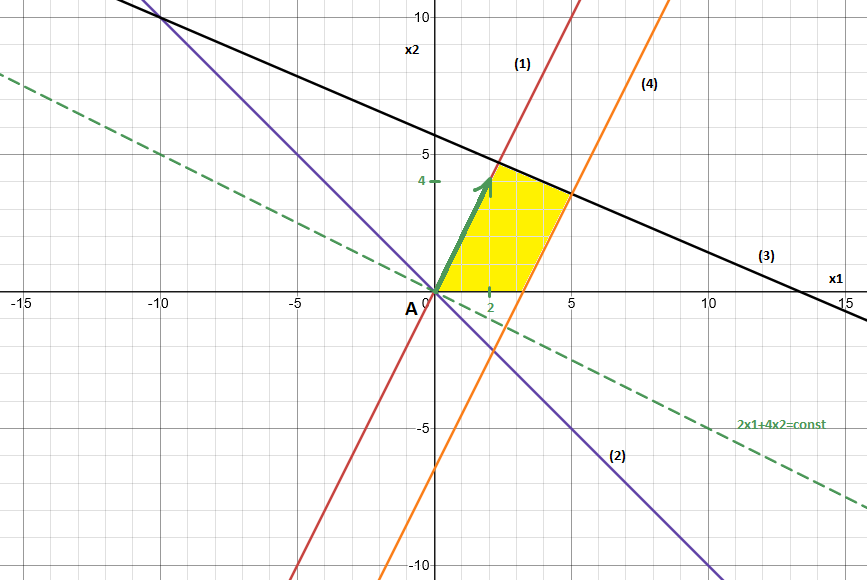
\includegraphics[width=\textwidth]{1-1.png}
\begin{center}
  Рис. 1.2 Область допустимых решений
\end{center}

Для линий уровня $2x_1+4x_2 = \text{const}$ строим нормальный вектор $\vec{n} = (2,4)$ перпендикулярно вектору нормаль построим одну из линий уровня Перемещаем её в направлении вектора $\vec{n}$ до опорной прямой. Для определения координат точки A решаем систему уравнений:\\

\begin{math}
  \begin{cases}
    2x_1-x_2 \geq 0,(1)\\
    -x_1-x_2 \leq 0,(2)\\
  \end{cases}
\end{math}\\

Получаем $x_1 = 0, x_2 = 0$ это и есть оптимальное решение. Минимальное значение целевой функции $Z(X) = 2 \cdot 0 + 4 \cdot 0 = 0$.
\newpage
\section{Транспортная задача}
\subsection{Краткие теоретические сведения по теме лабораторной работы}
Транспортная задача (ТЗ) — одна из распространенных задач линейного программирования. Ее цель — разработка наиболее рациональных путей и способов транспортирования товаров, устранение чрезмерно дальних, встречных, повторных перевозок. 

Задана матрица $c=(c_{ij})$ транспортных расходов: затраты на перевозку единицы продукции из пункта производства i в пункт потребления j.

Требуется составить план перевозок, который не выводит за пределы мощностей производителей, удовлетворяет полностью всех потребителей и минимизирует суммарные затраты на перевозки.

\underline{Постановка задачи:} Пусть имеется m пунктов производства и n пунктов потребления одного продукта. Объем производства в пункте производства с номером i равен $а_i$, объём потребления в пункте потребления с номером j равен $b_j, (i=1,2,…,m; j= 1,2,…n)$.

Введем обозначение: $х_{ij}$ — количество груза, которое нужно перевезти из i-го пункта отправления в j-й пункт назначения. Так как нужно перевезти весь груз из каждого пункта отправления $а_i$‚ то должны выполняться равенства:\\

\begin{math}
  \begin{cases}
    x_{11}+x_{12}+\ldots+x_{1n}=a_1\\
    \ldots\\
    x_{m1}+x_{m2}+\ldots+x_{mn}=a_m\\
  \end{cases}
\end{math}\\

Размер поставок должен выражаться неотрицательным числом: $x_{ij}\geq0,i=\overline{1,m} ,j=\overline{1,n} $. Стоимость всех запланированный перевозок должна быть минимальной:
\begin{align*}
  F(x)= c_{11}x_{11}+\ldots+c_{mn}x_{mn}\rightarrow \min\\
  \begin{cases}
    x_{11}+\ldots+x_{m1} = b_1\\
    \ldots\\
    x_{1n}+\ldots+x_{mn} = b_n\\
  \end{cases}
\end{align*}

В рассмотренной модели ТЗ предполагается, что суммарные запасы поставщиков равны суммарным запросам потребителей. Такая задача называется задачей с правильным балансом (сбалансированной задачей), ее модель — закрытой. В противном случае транспортная задача линейного программирования называется открытой.


\subsection{Решение индивидуального задания}
\subsubsection{exel}
Дана задача \\
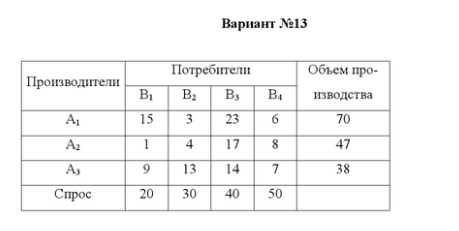
\includegraphics{2-1.png}\\
Создаем таблицу для ввода условий задачи и введем исходные данные:\\

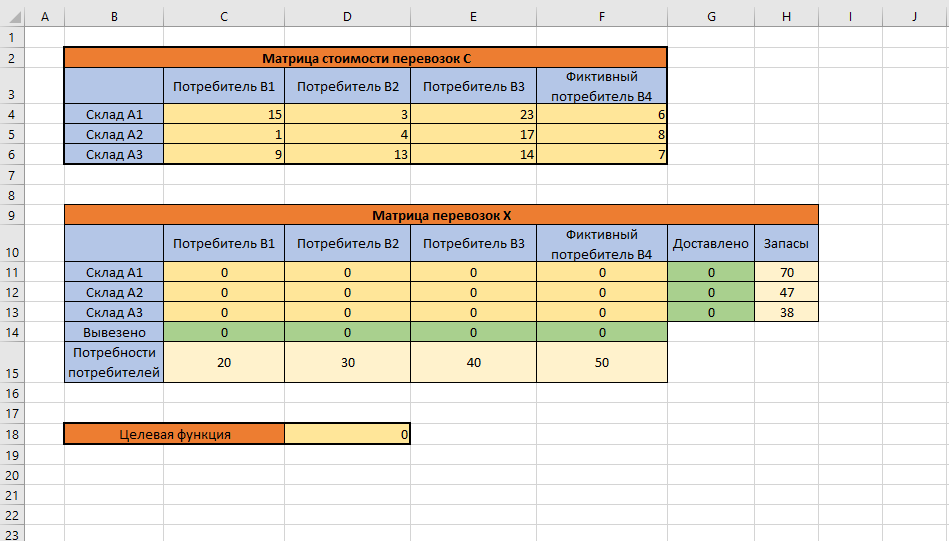
\includegraphics[width=\textwidth]{2-2.png}\\

Вводим формулы расчета для различных ячеек:
\begin{verbatim}
  D18 =SUMPRODUCT(C4:F6;C11:F13)

  G11 =SUM(C11:F11)
  G12 =SUM(C12:F12)
  G13 =SUM(C13:F13)

  C14 =SUM(C11:C13)
  D14 =SUM(D11:D13)
  E14 =SUM(E11:E13)
  F14 =SUM(F11:F13)
\end{verbatim}

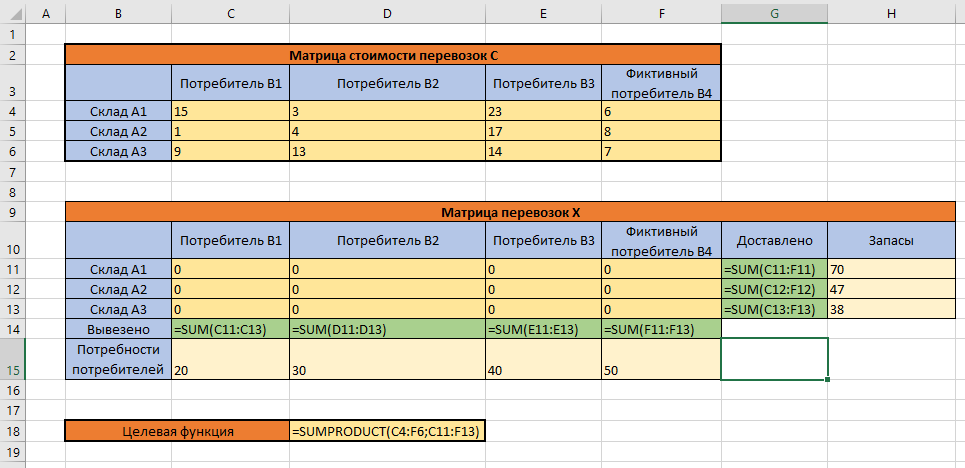
\includegraphics[width=\textwidth]{2-3.png}\\

\newpage
Заполняем окно параметров поиска решений:\\

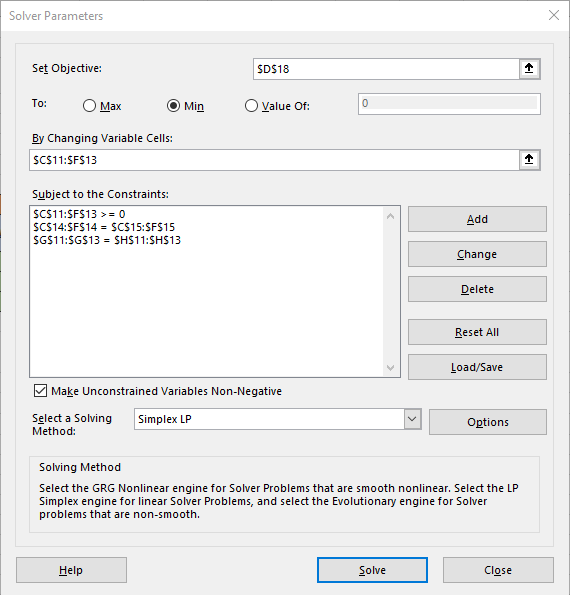
\includegraphics{2-4.png}\\

Результат: \\

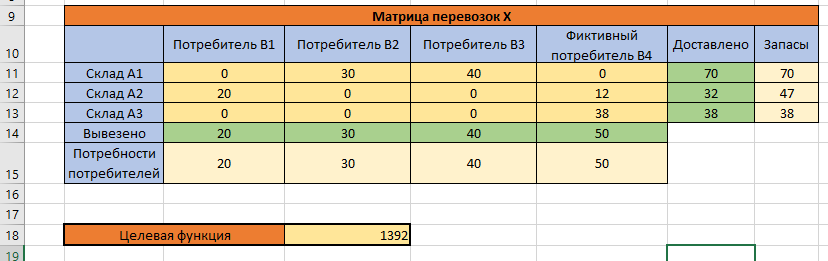
\includegraphics[width=\textwidth]{2-5.png}\\
\subsubsection{Метод потенциалов(опорный план с помощью северо-западного угла)}

Задана таблица транспортной задачи:
\begin{table}[H]
\centering
\begin{tabular}{c|c|c|c|c|}
\cline{2-5}
                              & B1=20 & B2=30 & B3=40 & B4=50 \\ \hline
\multicolumn{1}{|c|}{A1 = 70} & 15    & 3     & 23    & 6     \\ \hline
\multicolumn{1}{|c|}{A2 = 47} & 1     & 4     & 17    & 8     \\ \hline
\multicolumn{1}{|c|}{A3 = 38} & 9     & 13    & 14    & 7     \\ \hline
\end{tabular}
\end{table}

Суммарные запасы груза $70+47+38=155$, а суммарное потребление $20+30+40+50=140$. Следовательно Задача является открытого типа и ее нужно закрыть вводом нового потребителя с стоимостью перевозок 0 и потребностями $155-140=15$.
\begin{table}[H]
\centering
\begin{tabular}{c|c|c|c|c|c|}
\cline{2-6}
                              & B1=20 & B2=30 & B3=40 & B4=50 & B5=15 \\ \hline
\multicolumn{1}{|c|}{A1 = 70} & 15    & 3     & 23    & 6     & 0     \\ \hline
\multicolumn{1}{|c|}{A2 = 47} & 1     & 4     & 17    & 8     & 0     \\ \hline
\multicolumn{1}{|c|}{A3 = 38} & 9     & 13    & 14    & 7     & 0     \\ \hline
\end{tabular}
\end{table}

Метод северо-западного угла:
\begin{table}[H]
\centering
\begin{tabular}{|c|c|c|c|c|c|c|}
\hline
            & B1      & B2    & B3    & B4    & B5    & Запасы \\ \hline
A1          & 15[20]  & 3[30] & 23[20]& 6[0]  & 0[0]  & 70     \\ \hline
A2          & 1[0]    & 4[0]  & 17[20]& 8[27] & 0[0]  & 47     \\ \hline
A3          & 9[0]    & 13[0] & 14[0] & 7[23] & 0[15] & 38     \\ \hline
Потребности & 20      & 30    & 40    & 50    & 15    &        \\ \hline
\end{tabular}
\end{table}

\begin{math}
  7 = m+n-1 = 3+5-1 = 7 \Rightarrow \textsc{невырожденный}\\
  F(x)=\sum_{i=1}^3\sum_{j=1}^5 c_{ij}x_{ij} = 15\cdot20+3\cdot30+23\cdot20+17\cdot20+8\cdot27+7\cdot23+0\cdot15 = 1567
\end{math}\\

Метод потенциалов:\\
1. Находим предварительные потенциалы $u_i,v_j$, по заданному плану, где $u_i+v_j=c_{ij}, u_1 = 0$\\
2. Проверяем на оптимальность, где не существуют $u_i+v_j > c_{ij}$ \\
3. Выбераем максимальную оценку свобдной клетки\\
4. Строим цикл, чередуя +/-, вершина цикла, выбранная свободная клетка начинается с '+', выбераем наименьшей объем груза из ячеек с '-', и прибавляем это значение к элементам цикла\\

\newpage
1-итерация:\\
\begin{equation*}
  1)\begin{split}
    u_1 + v_1 = 15; v_1 = 15-0 = 15\\
    u_1 + v_2 = 3; v_2 = 3-0 = 3\\
    u_1 + v_3 = 23; v_3 = 23-0 = 23\\
    u_2 + v_3 = 17; u_2 = 17-23 = -6\\
    u_2 + v_4 = 8; v_4 = 8-(-6) = 14\\
    u_3 + v_4 = 7; u_3 = 7-14 = -7\\
    u_3 + v_5 = 0; v_5 = 0-(-7) = 7\\
  \end{split}
  \qquad  
  2)\begin{split}
    \Delta_{14} = 0 + 14 - 6 = 8 > 0 \\
    \Delta_{15} = 0 + 7 - 0 = 7 > 0 \\
    \Delta_{21} = -6 + 15 - 1 = 8 > 0 \\
    \Delta_{22} = -6 + 3 - 4 = -7 < 0 \\
    \Delta_{25} = -6 + 7 - 0 = 1 > 0 \\
    \Delta_{31} = -7 + 15 - 9 = -1 < 0 \\
    \Delta_{32} = -7 + 3 - 13 = -17 < 0 \\
    \Delta_{33} = -7 + 23 - 14 = 2 > 0 \\
  \end{split}
\end{equation*}

\begin{math}
  3) \max(8,7,8,1,2)= 8 \Rightarrow \max(1_{21},6_{14}) = 6
\end{math}
\begin{table}[H]
\centering
\begin{tabular}{|c|c|c|c|c|c|c|}
\hline
            & B1(V1=15)& B2(V2=3) & B3(V3=23) & B4(V4=14) & B5(V5=7)  & Запасы \\ \hline
A1(U1=0)    & 15[20]   & 3[30]    & 23[20]-   & 6[0]+     & 0[0]      & 70     \\ \hline
A2(U2=-6)   & 1[0]     & 4[0]     & 17[20]+   & 8[27]-    & 0[0]      & 47     \\ \hline
A3(U3=-7)   & 9[0]     & 13[0]    & 14[0]     & 7[23]     & 0[15]     & 38     \\ \hline
Потребности & 20       & 30       & 40        & 50        & 15        &        \\ \hline
\end{tabular}
\end{table}

\begin{center}
  $\Downarrow$\\
  4) $(1,4)\rightarrow(1,3)\rightarrow(2,3)\rightarrow(2,4)\rightarrow(1,4)$\\
  $\min(20,27) = 20$
\end{center}
\begin{table}[H]
\centering
\begin{tabular}{|c|c|c|c|c|c|c|}
\hline
            & B1(V1=15)& B2(V2=3) & B3(V3=23) & B4(V4=14) & B5(V5=7)  & Запасы \\ \hline
A1(U1=0)    & 15[20]   & 3[30]    & 23[0]     & 6[20]     & 0[0]      & 70     \\ \hline
A2(U2=-6)   & 1[0]     & 4[0]     & 17[40]    & 8[07]     & 0[0]      & 47     \\ \hline
A3(U3=-7)   & 9[0]     & 13[0]    & 14[0]     & 7[23]     & 0[15]     & 38     \\ \hline
Потребности & 20       & 30       & 40        & 50        & 15        &        \\ \hline
\end{tabular}
\end{table}

2-итерация:\\
\begin{equation*}
  1)\begin{split}
    u_1 + v_1 = 15; v_1 = 15-0 = 15\\
    u_1 + v_2 = 3; v_2 = 3-0 = 3\\
    u_1 + v_4 = 6; v_4 = 6-0 = 6\\
    u_2 + v_4 = 8; u_2 = 8-6 = 2\\
    u_2 + v_3 = 17; v_3 = 17-2 = 15\\
    u_3 + v_4 = 7; u_3 = 7-6 = 1\\
    u_3 + v_5 = 0; v_5 = 0-1 = -1\\
  \end{split}
  \qquad  
  2)\begin{split}
    \Delta_{13} = 0 + 15 - 23 = -8 < 0 \\
    \Delta_{15} = 0 + (-1) - 0 = -1 < 0 \\
    \Delta_{21} = 2 + 15 - 1 = 16 > 0 \\
    \Delta_{22} = 2 + 3 - 4 = -1 < 0 \\
    \Delta_{25} = 2 + -1 - 0 = 1 > 0 \\
    \Delta_{31} = 1 + 15 - 9 = 7 > 0 \\
    \Delta_{32} = 1 + 3 - 13 = -9 < 0 \\
    \Delta_{33} = 1 + 15 - 14 = 2 > 0 \\
  \end{split}
\end{equation*}

\begin{math}
  3) \max(16,1,7,2)= 16 \Rightarrow \max(16_{21}) = 1
\end{math}
\begin{table}[H]
\centering
\begin{tabular}{|c|c|c|c|c|c|c|}
\hline
            & B1(V1=15)& B2(V2=3) & B3(V3=15) & B4(V4=6)  & B5(V5=-1) & Запасы \\ \hline
A1(U1=0)    & 15[20]-  & 3[30]    & 23[20]    & 6[0]+     & 0[0]      & 70     \\ \hline
A2(U2=2)    & 1[0]+    & 4[0]     & 17[40]    & 8[7]-     & 0[0]      & 47     \\ \hline
A3(U3=1 )   & 9[0]     & 13[0]    & 14[0]     & 7[23]     & 0[15]     & 38     \\ \hline
Потребности & 20       & 30       & 40        & 50        & 15        &        \\ \hline
\end{tabular}
\end{table}

\begin{center}
  $\Downarrow$\\
  4) $(2,1)\rightarrow(1,1)\rightarrow(1,4)\rightarrow(2,4)\rightarrow(2,1)$\\
  $\min(20,7) = 7$
\end{center}
\begin{table}[H]
\centering
\begin{tabular}{|c|c|c|c|c|c|c|}
\hline
     & B1       & B2       & B3)       & B4        & B5        & Запасы \\ \hline
A1   & 15[13]   & 3[30]    & 23[0]     & 6[27]     & 0[0]      & 70     \\ \hline
A2   & 1[7]     & 4[0]     & 17[40]    & 8[0]      & 0[0]      & 47     \\ \hline
A3   & 9[0]     & 13[0]    & 14[0]     & 7[23]     & 0[15]     & 38     \\ \hline
Потребности & 20       & 30       & 40        & 50        & 15        &        \\ \hline
\end{tabular}
\end{table}

3-итерация:\\
\begin{equation*}
  1)\begin{split}
    u_1 + v_1 = 15; v_1 = 15-0 = 15\\
    u_2 + v_1 = 1; u_2 = 1-15 = -14\\
    u_2 + v_3 = 17; v_3 = 17+14 = 31\\
    u_1 + v_2 = 3; v_2 = 3-0 = 3\\
    u_1 + v_4 = 6; v_4 = 6-0 = 6\\
    u_3 + v_4 = 7; u_3 = 7-6 = 1\\
    u_3 + v_5 = 0; v_5 = 0-1 = -1\\
  \end{split}
  \qquad  
  2)\begin{split}
    \Delta_{13} = 0+31-23= 8 > 0 \\
    \Delta_{31} = 1+15-9= 7 > 0 \\
    \Delta_{33} = 1+31-14= 18 > 0 \\
  \end{split}
\end{equation*}

\begin{math}
  3) \max(8,7,18)= 18 \Rightarrow \max(18_{33}) = 14
\end{math}
\begin{table}[H]
\centering
\begin{tabular}{|c|c|c|c|c|c|c|}
\hline
            & B1(V1=15)& B2(V2=3) & B3(V3=31) & B4(V4=6)  & B5(V5=-1) & Запасы \\ \hline
A1(U1=0)    & 15[13]-  & 3[30]    & 23[0]     & 6[27]+    & 0[0]      & 70     \\ \hline
A2(U2=-14)  & 1[7]+    & 4[0]     & 17[40]-   & 8[0]      & 0[0]      & 47     \\ \hline
A3(U3=1 )   & 9[0]     & 13[0]    & 14[0]+    & 7[23]-    & 0[15]     & 38     \\ \hline
Потребности & 20       & 30       & 40        & 50        & 15        &        \\ \hline
\end{tabular}
\end{table}

\begin{center}
  $\Downarrow$\\
  4) $(3,3)\rightarrow(2,3)\rightarrow(2,1)\rightarrow(1,1)\rightarrow(1,4)\rightarrow(3,4)\rightarrow(3,3)$\\
  $\min(13,23,40) = 13$
\end{center}
\begin{table}[H]
\centering
\begin{tabular}{|c|c|c|c|c|c|c|}
\hline
     & B1       & B2       & B3        & B4        & B5        & Запасы \\ \hline
A1   & 15[0]    & 3[30]    & 23[0]     & 6[40]     & 0[0]      & 70     \\ \hline
A2   & 1[20]    & 4[0]     & 17[27]    & 8[0]      & 0[0]      & 47     \\ \hline
A3   & 9[0]     & 13[0]    & 14[13]    & 7[10]     & 0[15]     & 38     \\ \hline
Потребности & 20       & 30       & 40        & 50        & 15        &        \\ \hline
\end{tabular}
\end{table}

4-итерация:\\
\begin{equation*}
  1)\begin{split}
    v_2= 3 - u_1 = 3-0 = 3\\
    v_4= 6 - u_1 = 6-0 = 6\\
    u_3= 7 - v_4 = 7-6 = 1\\
    v_3= 14 - u_3 = 14-1 = 13\\
    u_2= 17 - v_3 = 17-13 = 4\\
    v_1= 1 - u_2 = 1-4 = -3\\
    v_5= 0 - u_3 = 0-1 = -1\\
  \end{split}
  \qquad  
  2)\begin{split}
    \Delta_{22} =4+3-4=3> 0 \\
    \Delta_{24} =4+6-8=2> 0 \\
    \Delta_{25} =4-1-0=3> 0 \\
  \end{split}
\end{equation*}

\begin{math}
  3) \max(3,2,3)= 3 \Rightarrow \max(3_{22}) = 4
\end{math}
\begin{table}[H]
\centering
\begin{tabular}{|c|c|c|c|c|c|c|}
\hline
            & B1(V1=-3)& B2(V2=3) & B3(V3=13) & B4(V4=6)  & B5(V5=-1) & Запасы \\ \hline
A1(U1=0)    & 15[0]    & 3[30]-   & 23[0]     & 6[40]+    & 0[0]      & 70     \\ \hline
A2(U2=4)    & 1[20]    & 4[0]+    & 17[27]-   & 8[0]      & 0[0]      & 47     \\ \hline
A3(U3=1 )   & 9[0]     & 13[0]    & 14[13]+   & 7[10]-    & 0[15]     & 38     \\ \hline
Потребности & 20       & 30       & 40        & 50        & 15        &        \\ \hline
\end{tabular}
\end{table}

\begin{center}
  $\Downarrow$\\
  4) $(2,2)\rightarrow(1,2)\rightarrow(1,4)\rightarrow(3,4)\rightarrow(3,3)\rightarrow(2,3)\rightarrow(2,2)$\\
  $\min(30,10,27) = 10$
\end{center}
\begin{table}[H]
\centering
\begin{tabular}{|c|c|c|c|c|c|c|}
\hline
     & B1       & B2       & B3        & B4        & B5        & Запасы \\ \hline
A1   & 15[0]    & 3[20]    & 23[0]     & 6[50]     & 0[0]      & 70     \\ \hline
A2   & 1[20]    & 4[10]    & 17[17]    & 8[0]      & 0[0]      & 47     \\ \hline
A3   & 9[0]     & 13[0]    & 14[23]    & 7[0]      & 0[15]     & 38     \\ \hline
Потребности & 20       & 30       & 40        & 50        & 15        &        \\ \hline
\end{tabular}
\end{table}

5-итерация:\\
\begin{equation*}
  1)\begin{split}
    v_2= 3 - u_1 = 3-0 = 3\\
    u_2= 4 - v_2 = 4-3 = 1\\
    v_1= 1 - u_2 = 1-1 = 0\\
    v_3= 17 - u_2 = 17-1 = 16\\
    u_3= 14 - v_3 = 14-16 = -2\\
    v_5= 0 - u_3 = 0+2 = 2\\
    v_4= 6 - u_1 = 6-0 = 6\\
  \end{split}
  \qquad  
  2)\begin{split}
    \Delta_{15} =0+2-0=2> 0 \\
    \Delta_{25} =1+2-0=3> 0 \\
  \end{split}
\end{equation*}

\begin{math}
  3) \max(2,3)= 3 \Rightarrow \max(3_{25}) = 0
\end{math}
\begin{table}[H]
\centering
\begin{tabular}{|c|c|c|c|c|c|c|}
\hline
            & B1(V1=0 )& B2(V2=3) & B3(V3=16) & B4(V4=6)  & B5(V5=2 ) & Запасы \\ \hline
A1(U1=0)    & 15[0]    & 3[20]    & 23[0]     & 6[50]     & 0[0]      & 70     \\ \hline
A2(U2=1)    & 1[20]    & 4[10]    & 17[17]-   & 8[0]      & 0[0]+     & 47     \\ \hline
A3(U3=-2)   & 9[0]     & 13[0]    & 14[23]+   & 7[0]      & 0[15]-    & 38     \\ \hline
Потребности & 20       & 30       & 40        & 50        & 15        &        \\ \hline
\end{tabular}
\end{table}

\begin{center}
  $\Downarrow$\\
  4) $(2,5)\rightarrow(3,5)\rightarrow(3,3)\rightarrow(2,3)\rightarrow(2,5)$\\
  $\min(17,15) = 15$
\end{center}
\begin{table}[H]
\centering
\begin{tabular}{|c|c|c|c|c|c|c|}
\hline
     & B1       & B2       & B3        & B4        & B5        & Запасы \\ \hline
A1   & 15[0]    & 3[20]    & 23[0]     & 6[50]     & 0[0]      & 70     \\ \hline
A2   & 1[20]    & 4[10]    & 17[2]     & 8[0]      & 0[15]     & 47     \\ \hline
A3   & 9[0]     & 13[0]    & 14[38]    & 7[0]      & 0[0]      & 38     \\ \hline
Потребности & 20       & 30       & 40        & 50        & 15        &        \\ \hline
\end{tabular}
\end{table}

6-итерация:\\
\begin{equation*}
  1)\begin{split}
    v_2= 3 - u_1 = 3-0 = 3\\
    u_2= 4 - v_2 = 4-3 = 1\\
    v_1= 1 - u_2 = 1-1 = 0\\
    v_3= 17 - u_2 = 17-1 = 16\\
    u_3= 14 - v_3 = 14-16 = -2\\
    v_5= 0 - u_2 = 0-1 = -1\\
    v_4= 6 - u_1 = 6-0 = 6\\
  \end{split}
  \qquad  
  2)\begin{split}
    \Delta_{11} = 0+0-15 \leq 0 \\
    \Delta_{13} = 0+16-23 = -7 \leq 0 \\
    \Delta_{15} = 0-1-0 = -1 \leq 0 \\
    \Delta_{24} = 1+6-8 = -1 \leq 0 \\
    \Delta_{31} = -2+0-0 = -11 \leq 0 \\
    \Delta_{32} = -2+3-13 = -12 \leq 0 \\
    \Delta_{34} = -2+6-7 = -3 \leq 0 \\
    \Delta_{35} = -2-1-0 = -3 \leq 0 \\
  \end{split}
\end{equation*}

\begin{table}[H]
\centering
\begin{tabular}{|c|c|c|c|c|c|c|}
\hline
     & B1       & B2       & B3        & B4        & B5        & Запасы \\ \hline
A1   & 15[0]    & 3[20]    & 23[0]     & 6[50]     & 0[0]      & 70     \\ \hline
A2   & 1[20]    & 4[10]    & 17[2]     & 8[0]      & 0[15]     & 47     \\ \hline
A3   & 9[0]     & 13[0]    & 14[38]    & 7[0]      & 0[0]      & 38     \\ \hline
Потребности & 20       & 30       & 40        & 50        & 15        &        \\ \hline
\end{tabular}
\end{table}

Опорный план является оптимальным, т.к. все оценки свободных клеток удовлетворяют условию $u_i+v_j\leq c_{ij}$. Затраты: $F(x)=3\cdot20+6\cdot50+1\cdot20+4\cdot10+17\cdot2+0\cdot15+14\cdot38 = 986$


\newpage
\section{Задача коммивояжера}
\subsection{Краткие теоретические сведения по теме лабораторной работы}
Имеется n городов. Расстояния между любой парой городов i и j известны и составляют c ij . Коммивояжер выезжает из какого-либо города и должен посетить все города, побывав в каждом только один раз и вернуться в исходный город. Ставится задача определить такую последовательность объезда городов, или маршрут, при которой суммарная длина маршрута была бы минимальной
\subsection{Решение индивидуального задания}
Дана задача (12 вариант, т.к. 13 нету):
\begin{table}[H]
\centering
\begin{tabular}{|c|c|c|c|c|c|c|c|c|c|c|c|c|c|c|c|c|c|c|c|}
\hline
a & b & c & d & e & f & g & h & k & m & n & p & q & r & s & t & x & y & z & w \\ \hline
8 & 5 & 15& 6 & 6 & 5 & 5 & 2 & 6 & 5 & 5 & 6 & 5 & 3 & 5 & 4 & 8 & 4 & 5 & 9 \\ \hline
\end{tabular}
\end{table}

Матрица растояний (C):
\begin{table}[H]
\centering
\begin{tabular}{c|c|c|c|c|c|}
  &n1      &n2      &n3      &n4      &n5      \\ \hline
n1&$\infty$&8       &5       &15      &6       \\ \hline
n2&6       &$\infty$&5       &5       &2       \\ \hline
n3&6       &5       &$\infty$&5       &6       \\ \hline
n4&5       &3       &5       &$\infty$&4       \\ \hline
n5&8       &4       &5       &9       &$\infty$\\ \hline
\end{tabular}
\end{table}

\newpage
\subsection{MS Exel}
Начнём работу в электронной таблице MS Exсel. Создадим на листе матрицу состояний C, заполнив её исходными данными:\\

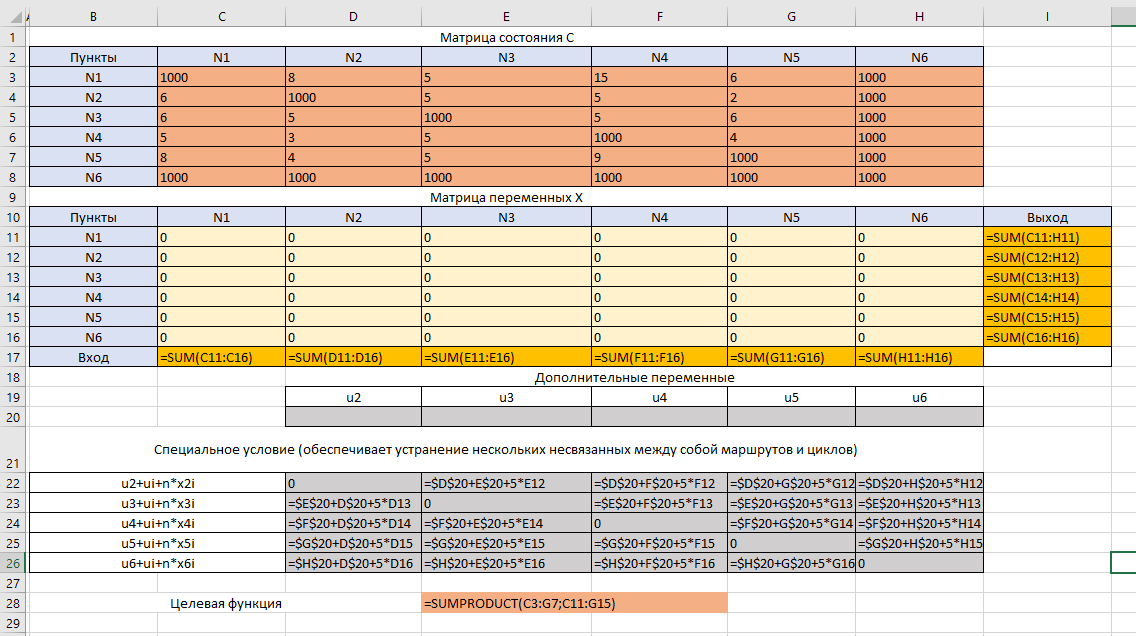
\includegraphics[width=\textwidth]{3-1.png}\\

Матрицу переменных X заполняем нулями 

В ячейку C16 запишем формулу: =СУММ(C11:C15). Автозаполнением скопируем эту формулу в ячейки диапазона D16:G16. 

В ячейку H11 запишем формулу: =СУММ(C11:G11). Автозаполнением скопируем эту формулу в ячейки диапазона H12:15. 

В ячейку F28 вводим формулу целевой функции: =СУММПРОИЗВ(C3:G7;C11:G15). В ячейки диапазона D22:G25 вводим формулы, соответствующие ограничениям: 
\begin{itemize}
	\item В ячейку E22: =\$D\$20-E20+6*E12. Автозаполнением копируем формулу в ячейки F26,G26; 
	\item В ячейку D23: =\$E\$20-D20+6*D13. Автозаполнением копируем формулу в ячейки E23, G23; 
	\item В ячейку D24: =\$F\$20-D20+6*D14. Автозаполнением копируем формулу в ячейки E24, G24; 
	\item В ячейку D25: =\$G\$20-D20+6*D15. Автозаполнением копируем формулу в ячейки E25, G25. 
	\item Ячейки D22, E23, F24, G25 = 0.
\end{itemize}

На вкладке «Данные» выбираем пункт «Поиск решения». В появившемся окне «Параметры поиска решения» (рис.2) выполняем необходимые установки: 

В поле «Оптимизировать целевую функцию» вводим абсолютный адрес ячейки F28; Направление целевой функции устанавливаем «Минимум»; 

В поле «Изменяя ячейки переменных» вводим абсолютный адрес диапазона ячеек \\\$C\$11:\$G\$15;\$D\$20:\$G\$20;
\begin{enumerate}
\item\$C\$11:\$G\$15 = бинарное 
\item\$C\$16:\$G\$16 = 1 
\item\$D\$22:\$G\$25 <= 5 
\item\$H\$11:\$H\$15 = 1 
\end{enumerate}
Устанавливаем галочку «Сделать переменные без ограничений неотрицательными» и выбираем метод решения «Поиск решения линейных задач симплекс-методом».\\

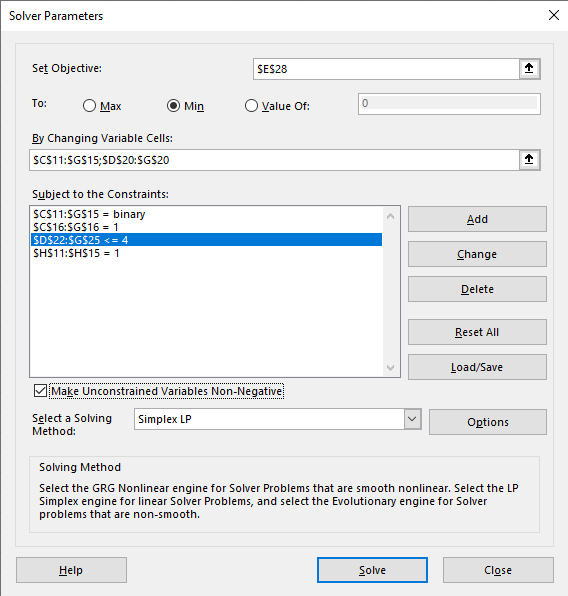
\includegraphics[width=\textwidth]{3-2.png}\\

\newpage
Нажимаем «Найти решение». Таким образом, путь:N1-N3-N4-N2-N5-N1. Минимальная длина маршрута 23.

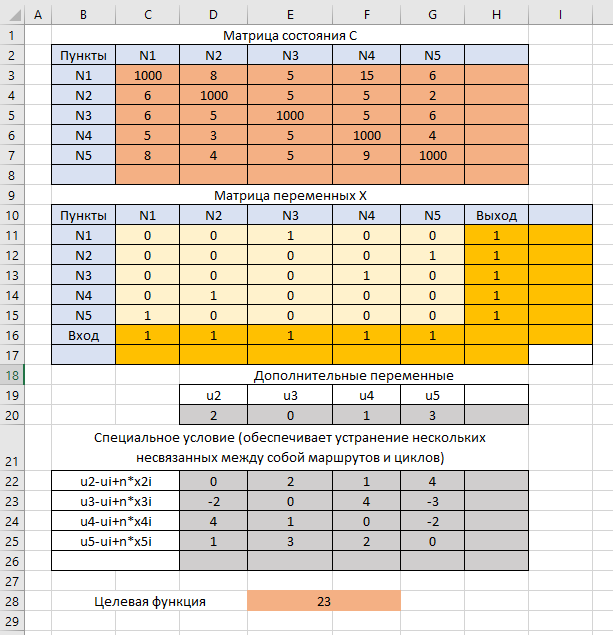
\includegraphics[width=\textwidth]{3-3.png}\\

\subsection{Вывод}
Задача коммивояжера может применяться для нахождения оптимального маршрута, позволяющего объехать определенные города по одному разу и вернуться в исходную точку.

\newpage
\section{Теория двойственности}
\subsection{Краткие теоретические сведения}
Любой задаче линейного программирования можно поставить в соответствие другую задачу которая называется двойственной или сопряженной. Общие правила составления двойственных задач: 
\begin{enumerate}
  \item Во всех ограничениях задачи свободные члены должны находиться в правой части, а члены с неизвестными в левой. 
  \item Ограничения-неравенства исходной задачи должны быть записаны так, чтобы знаки неравенств были направлены в одну сторону. 
  \item Если знаки неравенств в исходной задаче «=<»то целевая функция должна максимизироваться, иначе минимизироваться.
  \item Каждому ограничению исходной задачи соответствует неизвестное двойственной задачи. 
  \item Целевая функция двойственной задачи должна оптимизироваться противоположным образом по сравнению с целевой функцией исходной задачи. 
\end{enumerate}
\subsection{Постановка задачи. 13 вариант}
Составить и решить двойственную задачу и, используя ее решение, найти решение исходной задачи
\begin{align*}
  Z(X)=x_1+3x_2+\frac{2}{3}x_3 \rightarrow \min\\
  \begin{cases}
    x_1-2x_2+x_3 \geq 2,\\
    3x_1+x_2+x_3 \geq 3,\\
    2x_1+3x_2-x_3\geq 1,\\
  \end{cases}
  \qquad x_j \geq 0, j=1,2,3
\end{align*}

Составляем двойственную задачу:
\begin{align*}
  F(Y)=-2y_1+3y_2+y_3 \rightarrow \max\\
  \begin{cases}
    y_1+3y_2+2y_3 \leq 1\\
    -2y_1+y_2+3y_3 \leq 3\\
    y_1+y_2-y_3 \leq \frac{2}{3}\\
  \end{cases}
\end{align*}

Введем дополнительные переменные:
\begin{align*}
  F(Y)=-2y_1+3y_2+y_3+0y_4+0y_5+0y_6 \rightarrow \max\\
  \begin{cases}
    y_1+3y_2+2y_3+y_4 = 1\\
    -2y_1+y_2+3y_3+y_5 = 3\\
    y_1+y_2-y_3+y6 = \frac{2}{3}\\
  \end{cases} 
\end{align*}

Найдем решение нашей задачи с помощью симплекс метода
\begin{table}[H]
\centering
\begin{tabular}{|c|c|c|c|c|c|c|c|c|}
\hline
   & Y1 & \cellcolor[HTML]{FFCCC9}Y2 & Y3 & Y4 & Y5 & Y6 & Решение & Отношение \\ \hline
\rowcolor[HTML]{FFFC9E} 
Y4 & 1  & 3                          & 2  & 1  & 0  & 0  & 1       & 1/3       \\ \hline
Y5 & -2 & \cellcolor[HTML]{FFCCC9}1  & 3  & 0  & 1  & 0  & 3       & 3         \\ \hline
Y6 & 1  & \cellcolor[HTML]{FFCCC9}1  & -1 & 0  & 0  & 1  & 2/3     & 2/3       \\ \hline
Q  & 2 & \cellcolor[HTML]{FFCCC9}-3  & -1  & 0  & 0  & 0  & 0       &           \\ \hline
\end{tabular}
\end{table}

Результат 1 итерации
\begin{table}[H]
\centering
\begin{tabular}{|c|c|c|c|c|c|c|c|}
\hline
   & Y1   & Y2 & Y3   & Y4   & Y5 & Y6 & Решение \\ \hline
Y2 & 1/3  & 1  & 2/3  & 1/3  & 0  & 0  & 1/3     \\ \hline
Y5 & -7/3 & 0  & 7/3  & -1/3 & 1  & 0  & 8/3     \\ \hline
Y6 & 2/3  & 0  & -5/3 & -1/3 & 0  & 1  & 1/3     \\ \hline
Q  & 3    & 0  & 1    & 1    & 0  & 0  & 1       \\ \hline
\end{tabular}
\end{table}

В строке Q отсутствуют отрицательные элементы, следовательно оптимальный план найден за 1 итерацию. Оптимальное решение двойственно задачи: 
\begin{align*}
  y_1=0,\quad y_2=\frac{1}{3},\quad y_3=0\\
  Y=(0,\frac{1}{3},0)\\
  \max F(Y) = -2\cdot0+3\cdot\frac{1}{3}+1\cdot0
\end{align*}
Найдем оптимальное решение исходной задачи по формуле: $X_{j\text{опт}}^{\text{пр}} = -Q_{m+j}^{\text{дв}}$
\begin{align}
  x_1=-Q_{3+1}=-Q_4=1\\
  x_2=-Q_{3+2}=-Q_5=0\\
  x_3=-Q_{3+3}=-Q_6=0\\
  X=(1;0;0)\\
  \min Z(x)=1\cdot 1+3\cdot0+\frac{2}{3}\cdot0 = 1
\end{align}
\subsection{Вывод}
Научились решить двойственные задачи симплекс методом. Нашли оптимальное решение двойственной и исходной задач. Решение двойственных задач применяется в экономическом анализе
% 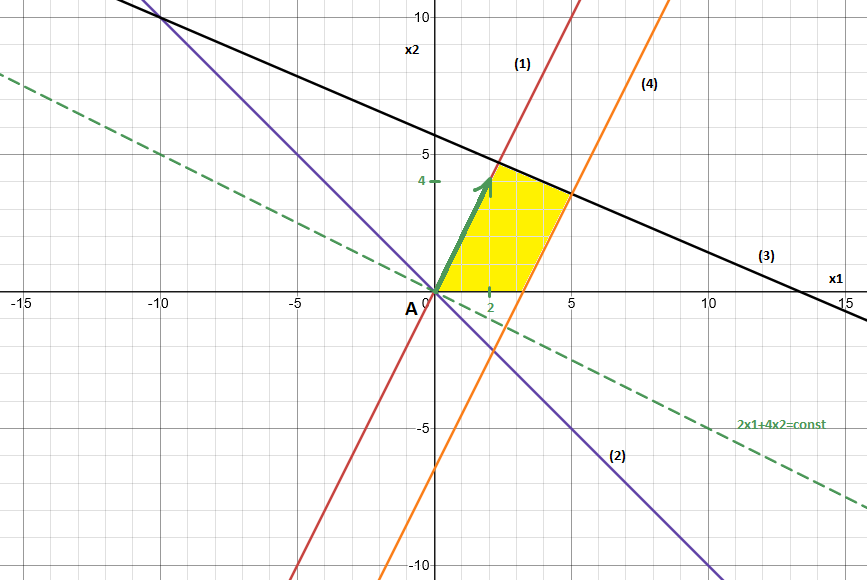
\includegraphics[width=\textwidth]{1-1.png}\\

\end{document}